\documentclass[a4paper,10pt]{article}

\usepackage{graphicx}
\usepackage{float}
\usepackage[utf8x]{inputenc} 
\usepackage[spanish]{babel}
\usepackage{hyperref}
\usepackage{listings}
\usepackage{verbatim}
\usepackage[top=2cm, bottom=1.5cm, left=2.5cm, right=1cm]{geometry}
\usepackage{pdfpages}
\usepackage{enumitem}
\usepackage{pdfpages}

\title{		\textbf{Trabajo Práctico N°1} \\Contador BCD de 4 dígitos con salida a display 7 segmentos }

\author{
            Tomás Boccardo, \textit{Padrón Nro. 93637}                     \\ 
            \texttt{tomasboccardo@gmail.com}                                              \\[4ex]
            \normalsize{2do. Cuatrimestre de 2013}                                      \\ [2.5ex]
            \normalsize{66.17 Sistemas Digitales}  \\
            \normalsize{Facultad de Ingeniería, Universidad de Buenos Aires}            \\ [3ex]
       }

\begin{document}

\maketitle
\thispagestyle{empty}   % quita el numero en la primer pagina
\newpage
\tableofcontents
\newpage
\section{Introdución}
El trabajo práctico consiste en diseñar, desarrollar, simular e implementar un contador BCD de 4 dígitos con salida a un display de  7 segmentos. En este informa se describirán los distintos pasos llevados a cabo para realización de el trabajo, así como las herramientas utilizadas para este fin.

\section{Diseño}
El siguiente diagrama de bloques fue diseñado basándose en el propuesto por la cátedra. La modificación que se introdujo fue remplazar los 4 contadores BCD de un solo dígito por un solo bloque con una salida de 4 bits por cada digito. Con esto se buscó encapsular mejor la implementación del contador, y así permitiendo abstraernos de su desarrollo.
	\begin{figure}[H]
		\centering
		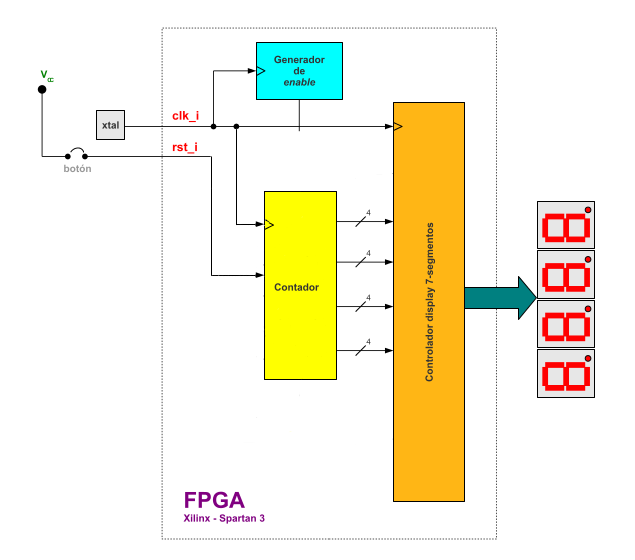
\includegraphics[scale=0.5]{diagBloques_global2.png}
		\caption{Diagrama de bloque de la arquitectura utilizada}
		\label{fig:diag_glob}
	\end{figure}
Como vemos, la arquitectura esta compuesta por tres bloques. A continuación se describirá cada uno con mayor detalle.
	\subsection{Generador de Enable}
	La función del generador de enable es la de dividir los pulsos del clock para enviar una señal a la entrada 'enable' del contador cada una dada cantidad de tiempo. Así se logra que el contador se incremente cada vez que se le enviá un pulso. \\
	Para cumplir con la función, implementaremos un contador que cuente determinada cantidad de pulsos del clock y llegada esa cantidad envíe un pulso de salida. Para hacerlo más genérico y fácil de testear, se decidió utilizar un genérico para poder variar la cantidad de pulsos a contar. Así mismo, como veremos en el diseño del controlador del display de 7 segmentos, también sera necesaria la utilización de un generador de enable por lo que, al hacerlo genérico se podrá reutilizar el ya desarrollado.
	\subsection{Controlador del display de 7 segmentos}
	La función del controlador del display de 7 segmentos es procesar la entrada de 4 dígitos representados en código binario y obtener una salida que alterne la selección del dígito del display y prenda los segmentos necesarios para representar el dígito en cuestión. Para esto se utilizara la arquitectura propuesta por la cátedra.
		\begin{figure}[H]
			\centering
			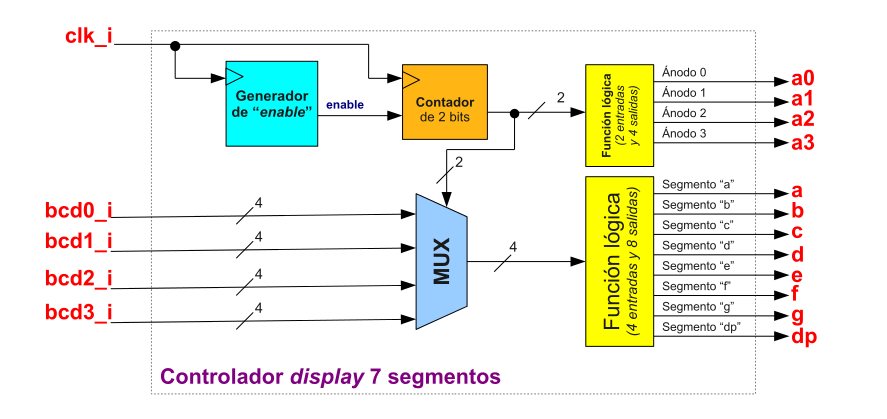
\includegraphics[scale=0.5]{diagBloques_contr.png}
			\caption{Diagrama de bloque de la arquitectura utilizada para el controlador de display}
			\label{fig:diag_contr}
		\end{figure}
	Como vemos en el diagrama, la arquitectura esta compuesta por 5 componentes.
		\subsubsection{Multiplexor}
		Su función es seleccionar cual de los dígitos de entrada (en formato BCD) se imprimirá en el display seleccionado. 
		\subsubsection{Función lógica de 4 entradas y 8 salidas}
		Se encarga de mapear el dígito de entrada a los segmentos correspondientes para su representación.
		\subsubsection{Función lógica de 2 entradas y 4 salidas}
		Es la encargada de seleccionar cual de los dígitos del display debe estar encendido según el valor del contador en ese momento.
		\subsubsection{Contador de 2 bits}
		Es el encargado de ir conmutando en ánodo para mantener los cuatro caracteres del display encendidos.						\subsubsection{Generador de enable}
		Genera una señal de enable para que la conmutación de ánodos no sea muy rápida. (aprox. 1kHz)

\section{Conclusiones}




\end{document}
